\documentclass[a4paper,12pt,oneside]{article}
\setlength{\columnsep}{10mm}

%Packages%
%Standard-Packages
\usepackage[left=3cm, right=2cm, top=2.5cm, bottom=2cm, headheight=15pt]{geometry}
\usepackage[main=english,german]{babel}
\usepackage{graphicx}
\usepackage{tabularx}
\usepackage{multirow}
\usepackage{color}
\usepackage{fancyhdr}
\usepackage{natbib}
\usepackage[utf8]{inputenc}
\usepackage{booktabs}
\usepackage{url}
\usepackage{setspace}
%
\usepackage{longtable}
\usepackage{blindtext}
\usepackage{lmodern}
\usepackage{caption}
\usepackage{pdflscape}
\usepackage{textcomp}
\usepackage{amssymb}
\usepackage{mathptmx}
\usepackage[T1]{fontenc}
\usepackage{amsfonts}
\usepackage{amsmath}
\usepackage[absolute]{textpos}
\usepackage{bibgerm}
\usepackage{enumitem}
\usepackage{eurosym}
\usepackage{svg}
    %\usepackage{filecontents}
\usepackage{titlesec}
\usepackage{float}
%\usepackage{subcaption}

%\usepackage{subfigure}
%\captionsetup[subfigure]{ font=normal, labelfont=bf, labelformat=brace, position=top}

\usepackage{colortbl}
\usepackage[justification=centering]{caption}
\usepackage{pdfpages}
\usepackage[hidelinks]{hyperref}
\usepackage{multicol}
\usepackage{wrapfig}
\usepackage{tabularx}
\usepackage{longtable} % For tables spanning multiple pages
%%Abkuerzungsverzeichnis
\usepackage{enumitem}
\usepackage[]{acronym}
\usepackage[titletoc]{appendix}
%%Abkuerzungsverzeichnis

\svgpath{{svg/}{/Users/lennartsacre/Uni/Thesis/Laborbericht/Figures/svg}}


%preamble

%Seitenlayout
\pagestyle{fancy}

\lhead{\nouppercase\leftmark}
\chead{} 
\rhead[\leftmark]{\thepage}

\lfoot{}
\cfoot{}
\rfoot{}

\renewcommand{\headrulewidth}{0.4pt}
\setlength{\parindent}{0pt}
\setstretch{1.5}

\pagestyle{empty}

\begin{document}

\begin{singlespace}
    \begin{center}
    \begin{tabular}{@{}p{\textwidth}@{}}

\begin{textblock*}{50mm}(20mm,15mm)
\includegraphics[height=2cm]{0 Title/UzK_logo_english_blue.jpg}
\end{textblock*}
\\
\vspace*{1cm}

\begin{center}
\LARGE{\textbf{Bachelorarbeit}}
\end{center}
\\

\begin{center}
\large{Bachelor Thesis\\ \vspace{3mm} Bachelor of Science} \\
\end{center}

\\
\begin{center}
\textbf{\Huge{University of Cologne}}
\end{center}
\\
\begin{center}
\large{\textbf{Institute for plant science\\ \vspace{2mm} B.Sc. Biologie}} 
\end{center}
\\

\begin{center}
\large{Vorgelegt von:\\ \textbf{Vorname Nachname}} \\
\large{\textbf{7369521}}\\
\end{center}

\\

\begin{center}
\begin{tabular}{lll}
\large{Erstprüfer:} & \large Prof. Dr.-Ing. XY\\
\\
\large{Zweitprüfer:} & \large Prof. Dr.-Ing. XY\\
\\
\\
\large{Ausgegeben am:}  & \large Ausgabedatum\\
\\
\large{Abgegeben am:}  & \large Abgabedatum\\
\\
\end{tabular}
\end{center}

\end{tabular}
\end{center}
\end{singlespace}


\newpage
\pagenumbering {Roman}
\pagestyle{plain}
\setcounter{page}{2} 
\input{Title/Eidesstaatliche erklärung.tex}



%\pagenumbering {Roman}
%\pagestyle{plain}
%\newpage
%\setcounter{page}{2} 
%\begin{singlespace}
 %   \vspace{10mm}
  %  \phantomsection\addcontentsline{toc}{section}{Abstract}
   % \LARGE{\textbf{Abstract}}
 %   \vspace{4mm}
  %  \par
  %  \normalsize{This is the abstract}
%\end{singlespace}


\newpage
\pagenumbering {Roman}
\pagestyle{plain}
\newpage
\setcounter{page}{3} 
\begin{singlespace}
    \vspace{10mm}
    \phantomsection\addcontentsline{toc}{section}{Abbreviations}
    \LARGE{\textbf{Abbreviations}}
    \normalsize{\begin{acronym}[SynCom]
    \acro{SynCom}{Synthetic Community}
    \acro{Bipo}{\textit{Bipolaris sorokiniana}}
    \acro{OD}{Optical density}
    \acro{TSA}{Tryptic Soy Agar}
    \acro{TSB}{Tryptic Soy Broth}

\end{acronym}}
\end{singlespace}

\cleardoublepage

\pagenumbering{gobble}
\begin{singlespace}
\renewcommand{\contentsname}{Table of contents}
\tableofcontents
\end{singlespace}
\cleardoublepage
\pagestyle{plain}

% Begin Main Part
\pagenumbering {arabic}
\pagestyle{fancy}
\renewcommand{\figurename}{Figure}
\section{Introduction}

\subsection{The Role of the Plant Microbiome}
In their natural environment, plants are in constant interaction with a diverse community of microorganisms, known as the plant microbiota. These include bacteria, fungi, archaea, viruses, and even protists, which colonize various plant surfaces such as roots, leaves, and stems, as well as the internal tissues.
The plant microbiome has been recognized as a crucial factor influencing plant health and productivity for more than a century \cite{berg2016Plant}.
Many functions of the plant microbiome are essential for plant health and development. For instance, during germination, the initial stage of a plant's life cycle, certain plants rely heavily on microorganisms. Mosses, some of the oldest land plants, depend on microbial interactions to kickstart their growth \cite{hornschuh2006Mossassociated}. 
Similarly, orchids require the assistance of fungi to germinate successfully \cite{jacquemyn2015Mycorrhizal}. 

The plant microbiome plays a vital role in both pathogen suppression and nutrient acquisition, particularly in the rhizosphere. Acting as a protective shield against soil-borne pathogens, it directly inhibits harmful microbes while priming the plant's immune system to enhance resistance \cite{berg2016Plant}. At the same time, rhizosphere microbial communities facilitate the solubilization and uptake of essential nutrients such as nitrogen, phosphorus, and iron, thereby directly contributing to plant growth, crop yields. Due to the coevolution and interdependence between plants and their associated microbes, the concept of the holobiont emerges, representing them as a unified ecological unit \cite{spooren2024PlantDriven}.

During germination, seed-associated microbes are most critical for the inital stages of microbiome development. After germination, however, soil microbes usually become the major constituents of the plant microbiome. 
These plant-microbe relationsships extend beyond passive colonization. Plants actively shape their microbiome. 
One of the most influential processes is the release of root exudates, a mixture of primary and secondary metabolites. Primary metabolites such as sugars, organic acids, and amino acids serve as nutrient sources, selectively attracting fast-growing and metabolically versatile microbes to the rhizosphere.
Secondary metabolites play a regulatory role by either promoting the growth of beneficial microbes or suppressing harmful ones. These include antimicrobial compounds that deter pathogens, signaling molecules that influence microbial behavior and even act directly against microbial effectors or compunds that create a toxic environment for the microbes
\cite{spooren2024PlantDriven}.

\subsection{The SynCom approach}
Understanding the complex web of plant-microbe interactions requires tools to study simplified microbial communities and their roles in the microbiome. A \ac{SynCom} consist of defined microbial strains assembled to model natural microbiomes. 
Using this approach, it becomes possible to study plant-microbe and microbe-microbe interactions under controlled conditions, enabling the identification of beneficial microbes and mechanisms that can enhance plant health and resilience. By combining different microbial taxa, a \ac{SynCom} enables the study of both synergistic and antagonistic relationships within microbial communities.
The \ac{SynCom} used in this study was created by isolating bacterial strains from the roots of barley (Hordeum vulgare), a host with a well-defined microbiota. Plants were grown in natural soil collected from the \textit{"Kölner Loch"} \footnotemark \footnotetext{Nick Dunken} near the Max Planck Institute, ensuring that the microbial community was representative of a realistic environment. Bacterial strains were isolated directly from barley roots, as microorganisms that interact most closely with plants are typically concentrated in this region.
The \ac{SynCom} was designed to include members of the core microbiota consistently associated with barley across diverse environments. The strains were selected based on their ecological relevance and potential functional roles in the microbiome, such as nutrient cycling, pathogen suppression, and plant growth promotion. The strains included in this study, representing a potential \ac{SynCom} for investigating interactions within the barley root microbiota, are listed in Table~\ref{tab:strains}.

\subsection{Research Gap and Objectives}
Synthetic communities have been widely utilized to investigate plant-microbe interactions, including in barley. Prior studies have demonstrated the potential of multiparte SynComs to protect barley against pathogens such as Bipolaris sorokiniana, enhance plant growth, and improve resilience to abiotic stresses like drought. Inter-kingdom SynComs that combine bacterial and fungal strains have further highlighted the synergistic potential of these communities in promoting plant health. \cite{mahdi2022Fungal}. These findings underscore the utility of SynComs in advancing our understanding of complex plant-microbe systems.

However, in the context of this project, initial experiments with the selected SynCom failed to yield a positive effect on barley plants. In fact, certain observations suggested potential negative impacts, raising questions about the dynamics within this specific SynCom. The precise interactions among the selected bacterial strains, as well as individual effect on the plant and the fungal pathogen, remain poorly understood.

Addressing these gaps could provide critical insights into the mechanisms driving these interactions, possibly enabling the development of an optimized SynCom that fosters plant growth and resilience. By identifying factors such as antagonistic interactions, pathogen-promoting effects, or direct negative impacts on the plant, this study lays the groundwork for designing a more effective microbial community tailored to enhance barley productivity.

This study focuses on a small but critical aspect of these questions by examining the individual effects of each strain. By identifying potential antagonistic interactions, pathogen-promoting effects, or negative impacts on the plant, this project aims to contribute to a better understanding of the SynCom dynamics. These findings may help further efforts to design a \ac{SynCom} with a more beneficial effect on barley growth.

\begin{table}[!ht]
    \caption{Bacterial Strains in the SynCom}
    \label{tab:strains}
    \centering
    \makebox[\textwidth][c]{ % Center the table within the page
        \resizebox{1.1\textwidth}{!}{
    \begin{tabularx}{\textwidth}{|>{\centering\arraybackslash}p{1.5cm}|X|>{\centering\arraybackslash}p{1cm}|>{\centering\arraybackslash}p{2cm}|>{\centering\arraybackslash}p{2cm}|>{\centering\arraybackslash}X|}
        \hline
        \textbf{Strain number} & \textbf{Genus} & \textbf{Gram} & \textbf{Genus enriched in GP} & \textbf{Genus \linebreak beneficial} & \textbf{TYGS} \\ \hline
        428 & Acidovorax & - & No & Yes & Not found \\ \hline
        459 & Ensifer & - & No & Yes & Ensifer canadensis \\ \hline
        638 & Cellulomonas & + & No & Yes & Not found \\ \hline
        978 & Nocardioides & + & No & Yes & Not found \\ \hline
        997 & Pseudomonas & - & Yes & Yes & Pseudomonas cedrina \\ \hline
        1080 & Devosia & - & No & Yes & Not found \\ \hline
        1101 & Shinella & - & No & Yes & Not found \\ \hline
        1114 & Galbitalea & + & No & unidentified & Not found \\ \hline
        1208 & F\_Micrococcaceae & + & No & Yes & Not found \\ \hline
        1234 & Neorhizobium & - & No & Yes & Not found \\ \hline
        1334 & Arthrobacter & + & No & Yes & Not found \\ \hline
        1338 & Chitinophaga & - & Yes & Yes & Not found \\ \hline
        1350 & Microbacterium & + & No & Yes & Not found \\ \hline
        1362 & Lysobacter & - & Yes & Yes & Not found \\ \hline
        1475 & Hydrogenophaga & - & No & Yes & Not found \\ \hline
        1533 & Lysobacter & - & Yes & Yes & Not found \\ \hline
        1692 & Sphingomonas & - & Yes & Yes & Not found \\ \hline
        1703 & Devosia & - & No & Yes & Not found \\ \hline
        1725 & Sphingomonas & - & Yes & Yes & Sphingomonas \linebreak lacusdianchii \\ \hline
        1790 & Sphingomonas & - & Yes & Yes & Not found \\ \hline
        1847 & Pseudomonas & - & Yes & Yes & Pseudomonas \linebreak chlororaphis \\ \hline
        2751 & Bacillus & + & No & Yes & Priestia megaterium \\ \hline
        2998 & Paenibacillus & - & No & Yes & Paenibacillus \linebreak humicus \\ \hline
        3044 & Pseudomonas & - & Yes & Yes & Not found \\ \hline
    \end{tabularx}
    }
}
    \par
    \vspace*{0.2cm}
    \raggedright
    \textbf{Description:} Bacterial strains used in the \ac{SynCom} for studying barley root microbiota interactions. Columns include (left to right): strain ID, genus, gram type, weather the strain was enriched in Golden Promise compared to Hit4, plant-beneficial status of the genus, and classification via the Type Strain Genome Server (TYGS). The strain numbers are arbitrary and were assigned in previous studies.
\end{table}
\section{Methods}

\subsection{Strain Selection}

\subsection{Overview of Experimental Design}
To investigate the interactions within the bacterial \ac{SynCom} and their effects on barley and \textit{Bipolaris sorokiniana} (hereafter referred to as Bipo), three distinct experiments were conducted:
\begin{enumerate}
    \item \textbf{Halo Assay}: Testing interactions within the bacterial \ac{SynCom}.
    \item \textbf{Bipo Assay}: Evaluating bacterial interactions with the fungal pathogen \ac{Bipo}.
    \item \textbf{In Planta Jar Assay}: Assessing the effects of individual bacterial strains on barley plants.
\end{enumerate}
Each experiment focused on a specific aspect of plant-microbe and microbe-microbe interactions.


\subsection{Halo Assay: Testing Interactions Within Strains}
The halo assay was adapted from the method described by Getzke et al. (2023) to assess antagonistic interactions between bacterial strains in the \ac{SynCom} \cite{getzke2023Cofunctioning}. 

Liquid cultures of each strain were grown in \ac{TSB} and standardized to an \ac{OD} of 1 at 600 nm. For each plate, 600 µL of bacterial culture at OD600 = 1 was added to 50 g of molten \ac{TSA} before solidifying to create base plates for the assay.

Drops of 10 µL of liquid bacterial cultures, diluted to OD600 = 0.1, were applied to the solidified plates, ensuring that each strain interacted with every other strain exactly once. Plates were incubated and inhibition halos around the droplets were measured to quantify antagonistic interactions. This approach,  has been shown to effectively study microbial community dynamics \cite{getzke2023Cofunctioning}.


\subsection{Bipo Assay: Testing Interactions with Bipo.}
The goal of the Bipo Assay was to determine whether bacterial strains in the \ac{SynCom} inhibited the growth of the fungal pathogen Bipolaris sorokiniana. For the assay, Bipolaris sorokiniana was stamped onto fresh CMBS plates to establish fungal growth. Drops of liquid bacterial cultures, prepared as described in the Halo Assay, were applied to the same plates in proximity to the fungal colony.

Plates were incubated at (temperature) for 6 days, and fungal growth inhibition was assessed by measuring inhibition zones and weather the fungus could grow over the bacterial colony. Negative controls should have included plates with Bipolaris sorokiniana alone, without bacterial addition.
% Add more specific details here.

\subsection{In Planta Jar Assay: Testing Effects on Barley Plants}
The Jar Assay was conducted to evaluate the effects of individual bacterial strains in the \ac{SynCom} on barley (\textit{Hordeum vulgare}) growth. Barley seedlings were inoculated with bacterial cultures and grown in jars under greenhouse conditions.

Barley seeds were germinated and transferred to jars containing a standard sterile growth medium (e.g., soil or sand). A single inoculation of liquid bacterial culture was applied to the seedlings, with each strain tested individually. Mock-treated plants, inoculated with sterile water instead of bacterial cultures, served as negative controls.

Plants were grown under standard greenhouse conditions appropriate for barley cultivation. This included adequate light, temperature, and humidity levels conducive to plant growth. Measurements were taken after an appropriate growth period, sufficient to assess the effects of the bacterial treatments on plant development.

The following plant growth parameters were measured:
\begin{itemize}
    \item Root weight
    \item Root length
    \item Shoot length
\end{itemize}

This setup allowed for the systematic assessment of the effects of each bacterial strain on plant growth and health.
% Add more specific details here.
\section{Results and Discussion}

This section summarizes the results obtained from the Halo Assay, BS Assay, and Jar Assay, focusing on bacterial interactions, fungal inhibition, and plant growth effects.

\par
The first set of data analyzed focused on the effects of different bacterial strains on the root weight and root length of barley plants. These results are visualized in \autoref{fig:root_weight_boxplot} and \autoref{fig:root_length_boxplot} respectively.
Both figures are sorted by the mean of the root weight to enable better comparison. 


\begin{figure}[H]
    \centering
    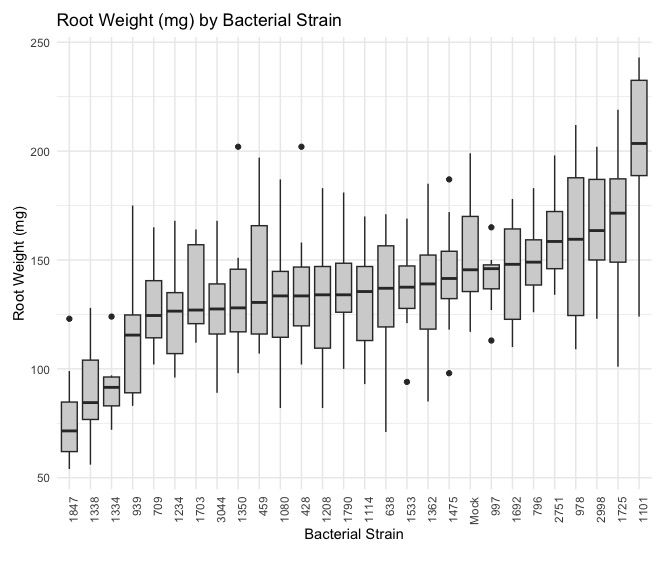
\includegraphics[width=0.8\linewidth]{Figures/Root Weight.jpeg}
    \caption{Root weight of barley after bacterial treatment.}
    \medskip
    \textbf{Description:} Distribution of root weight (in mg) for barley plants treated with different bacterial strains, sorted by the median root weight.
    \label{fig:root_weight_boxplot}
\end{figure}% Root Length Boxplot

\begin{figure}[H]
    \centering
    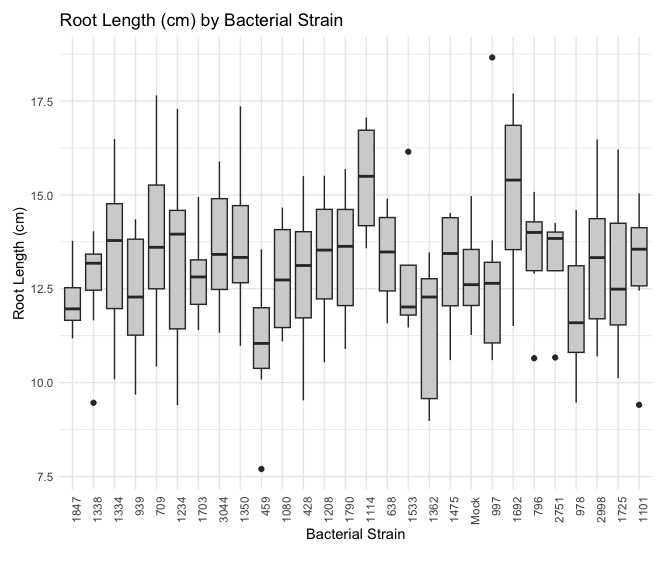
\includegraphics[width=0.8\linewidth]{Figures/RootLength.jpeg}
    \caption{Root length of barley after bacterial treatment.}
    \medskip
    \textbf{Description:} Distribution of root lengths (in cm) for barley plants treated with different bacterial strains, sorted by the median root weight.
    \label{fig:root_length_boxplot}
\end{figure}


The interactions between the bacterial strains, that were evaluated using the Halo Assay are visualized in \autoref{fig:heatmap} in the form of a heatmap. 
This heatmap represents the antagonistic effects observed between bacterial strains, where the size and color of the dots correspond to the size and strength of the inhibition halos, respectively. Small gray dots indicate the absence of halo, despite of bacterial growth, while the absence of a dot indicates no bacterial growth in that interaction. 

Some bacterial strains stood out by producing notably larger inhibition halos, indicating strong antagonistic effects. Most notably, strains 1208, 1847 consistently generated the largest halos, suggesting an ability to inhibit the growth of other strains. These strains displayed both substantial halo size and high halo strength, as represented by darker colors in \autoref{fig:heatmap}.

Certain bacterial strains were unable to establish growth when interacting with any of the other strains, as indicated by the absence of dots in \autoref{fig:heatmap}. This suggests that these strains were either highly sensitive to antagonistic effects from other strains or lacked the competitive ability to survive in such interactions under the experiment conditions. 
For example, strains 1114 and Y showed growth in only a few cases without producing measurable halos, suggesting a neutral or non-antagonistic role within the community.
% Heatmap
\begin{figure}[H]
    \centering
    \raggedright
    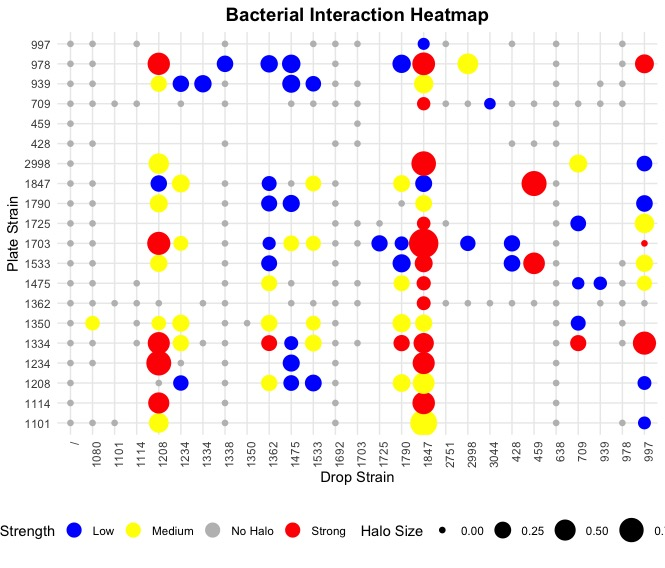
\includegraphics[width=\linewidth]{Figures/Heatmap.jpeg}
    \caption{Bacterial interaction heatmap}
    \medskip
    \textbf{Description:} Heatmap visualizing the interactions between bacterial strains, with halo size and strength indicating antagonistic effects. Grey dots represent no observed halo while the absence of a dot indicated no bacterial growth.
    \label{fig:heatmap}
\end{figure}

\begin{figure}[H]
    \centering
    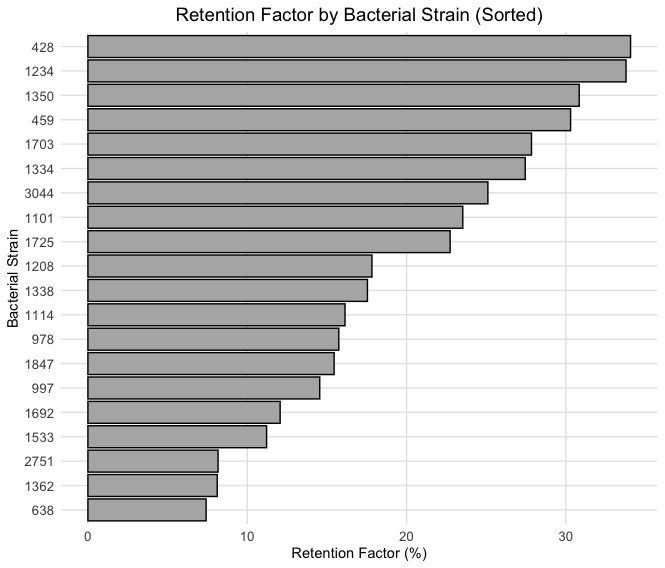
\includegraphics[width=\linewidth]{Figures/RetentionFactor.jpeg}
    \caption{Retention Factor by Bacterial Strain.}
    The retention factor measures the degree of inhibition caused by bacterial strains. 
    See the text below for details on the calculation.
    \label{fig:retention}
\end{figure}

\vspace{0.5cm} % Add space between the figure and the detailed explanation

\noindent
The retention factor is calculated using the formula:
\[
\text{Inhibition (\%)} = \frac{\text{Control Distance} - \text{Bacteria Distance}}{\text{Control Distance}} \times 100
\]
where the \textit{Control Distance} refers to the growth measurement in the absence of bacterial interference, and the \textit{Bacteria Distance} refers to the growth measurement in the presence of bacterial strains. Higher retention factor values indicate greater inhibition by the bacterial strain. The bar plot in \autoref{fig:retention} visualizes the retention factors for each bacterial strain, highlighting differences in inhibitory effects across strains.


Strain 1847 that was classified via the Type Strain Genome Server (TYGS), as can be seen in \autoref{tab:strains}, as \textit{Pseudomonas chlororaphis} conistently showed strong result across the three assay. This indicates a significant antagonistic avtivity towards other strains, effective inhibition of \ac{Bipo} growth and a notable influnce on root growth in the Jar Assay.

This strain was already subject of a study published in 2021 by Bertani et. al., showing several effect both on plant's and fungi. 
In the study, the \textit{Pseudomonas chlororaphis} strain effectively inhibited fungal pathogens like \textit{Fusarium graminearum} through antimicrobial production and colonized plant roots, enriching beneficial microbes in the rhizosphere. While it influenced plant stress pathways, it showed no direct growth-promotion effects under the tested conditions. \cite{bertani2021Isolation}

This correlated with our finings, as the strain reduced plant root growth and length while demonstrating  strong antagonistic effects on other bacterial strains and weak antagonistic effects on the fungal pathogen.

% End Main Part

\newpage
\pagestyle{plain}
\pagenumbering {Roman}
% List of Figures
\begin{singlespace}
    \newpage
    \setcounter{page}{3}
    \phantomsection
    \clearpage % Ensure no floating figures appear before this
    \addcontentsline{toc}{section}{List of Figures}
    \renewcommand{\listfigurename}{List of Figures}
    \listoffigures
    \vspace{3cm}
\end{singlespace}

% List of Tables
\begin{singlespace}
    \phantomsection
     % Ensure no floating tables appear before this
    \addcontentsline{toc}{section}{List of Tables}
    \renewcommand{\listtablename}{List of Tables}
    \listoftables
    \clearpage
\end{singlespace}


% Bibliography
\newpage
\bibliographystyle{apalike}
\phantomsection\addcontentsline{toc}{section}{Bibliography}
\renewcommand{\refname}{Bibliography}
\bibliography{References}
\newpage

% Appendix
\appendix
\appendixpage
\addappheadtotoc
    
\section*{Complete Medium for \textit{Bipolaris sorokiniana} (CM-Bs)}

CM-Bs medium was prepared as follows for 1 L:
\begin{itemize}[nosep]
    \item 10 mL Solution A
    \item 10 mL Solution B
    \item 0.5 mL Srb's micronutrients
    \item 0.5 mL FeCl solution
    \item 1 g Yeast extract
    \item 0.5 g Peptone
    \item 0.5 g Cassamine acids
    \item 10 g Glucose
    \item 15 g Agar (if solid medium is required)
\end{itemize}
The mixture was autoclaved before use.

\paragraph{Solution A (1 L)}
Dissolve 100 g $Ca(NO_3)_2 \cdot 4H_2O$ in MilliQ water and adjust the volume to 1 L. Store in the dark and shake well before use. Autoclave.
\\
\textbf{Solution B (1 L)}
Dissolve the following in 300 mL MilliQ water, combine, and adjust pH to 5.3 with NaOH:
\begin{itemize}[nosep]
    \item 20 g $KH_2PO_4$
    \item 25 g $MgSO_4 \cdot 7H_2O$
    \item 15 g $NaCl$
\end{itemize}
Add MilliQ water to 1 L, filter sterilize, store in the dark, and shake well before use.
\\
\textbf{Srb's Micronutrients (1 L):}
Dissolve the following:
\begin{itemize}[nosep]
    \item 57.2 mg $H_3BO_3$
    \item 393 mg $CuSO_4 \cdot 5H_2O$
    \item 13.1 mg KI
    \item 60.4 mg $MnSO_4 \cdot H_2O$
    \item 36.8 mg $(NH_4)_6Mo_7O_{24}$
    \item 5490 mg $ZnSO_4 \cdot H_2O$ or 8795.56 mg $ZnSO_4 \cdot 7H_2O$
\end{itemize}
Autoclave and store appropriately. 
\end{document}